\section{Graph Composer}
Un graf és un objecte matemàtic consisteix en un conjunt de vèrtex i arestes que els connecten. També és possible que coneguis els grafs sota el nom de xarxes. Cada vèrtex té diversos atributs o valors en funció del que s'està modelant. Les arestes poden tenir direccions i en aquests casos parlem de grafs dirigits.

El mòdul Graph Composer ofereix la possibilitat de fer música amb el pas per un graf. Cada vèrtex s'associa amb una nota i la seva duració en el temps. Les arestes que connecten els vèrtexs defineixen un camí pel què es pot viatjar a amb el temps. Això signigica que les notes es toquen en l'ordre dels vèrtexs visitats. El so que s'obté de cada vèrtex té diferents formes en funció del decorador del vèrtex, com ara una nota pura, un acord o un arpegi.

Per exemple, la següent partitura:
\begin{figure}[h]
\centering
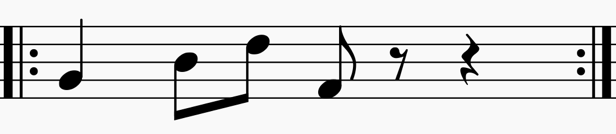
\includegraphics[width=0.5\textwidth]{GraphComposer_1}
\end{figure}

Es pot dibuixar com el següent graf dirigit:

\begin{figure}[h]
\centering
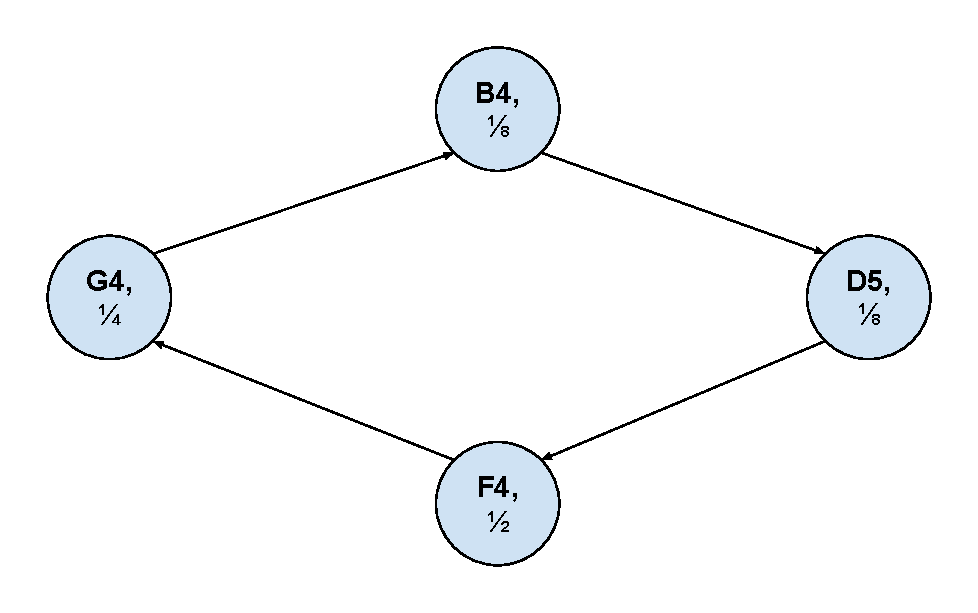
\includegraphics[width=0.5\textwidth]{GraphComposer_2}
\end{figure}

Els camins al graf representen seqüències de notes. Si el camí té un bucle, com a l'exemple d'abans, hi ha la repetició del fragment. A l'exemple, el graf té només un camí possible, però ,quan hi ha més d'una aresta sortint d'un vèrtex, hi ha diversos camins possibles.

Per exemple, el graf que veuràs a continuació té dos possibles camins:

\begin{figure}[h]
\centering
\begin{subfigure}{0.45\textwidth}
\centering
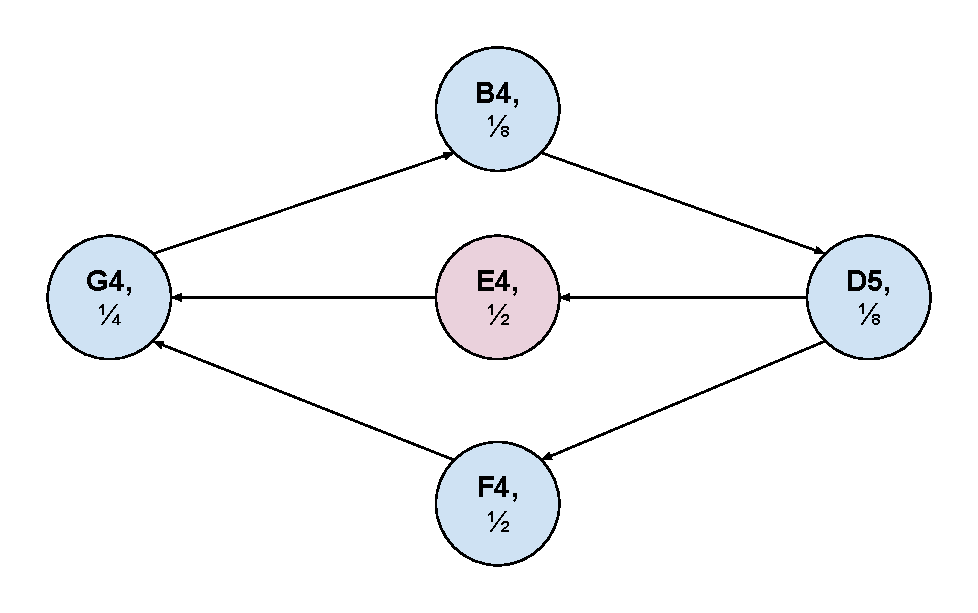
\includegraphics[height=3cm]{GraphComposer_3}
%\subcaption*{This graph can be walked through two paths.}
\end{subfigure}

\begin{subfigure}{0.45\textwidth}
\centering
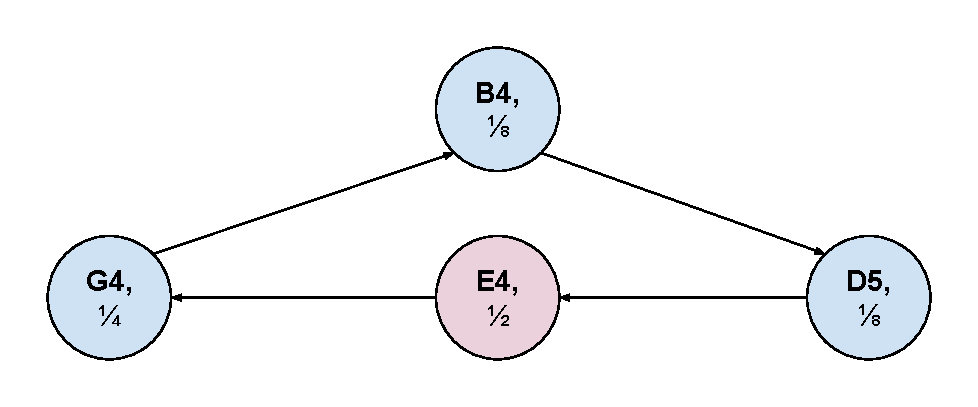
\includegraphics[width=\textwidth]{GraphComposer_5}
%\subcaption*{First path.}
\end{subfigure}
\begin{subfigure}{0.45\textwidth}
\centering
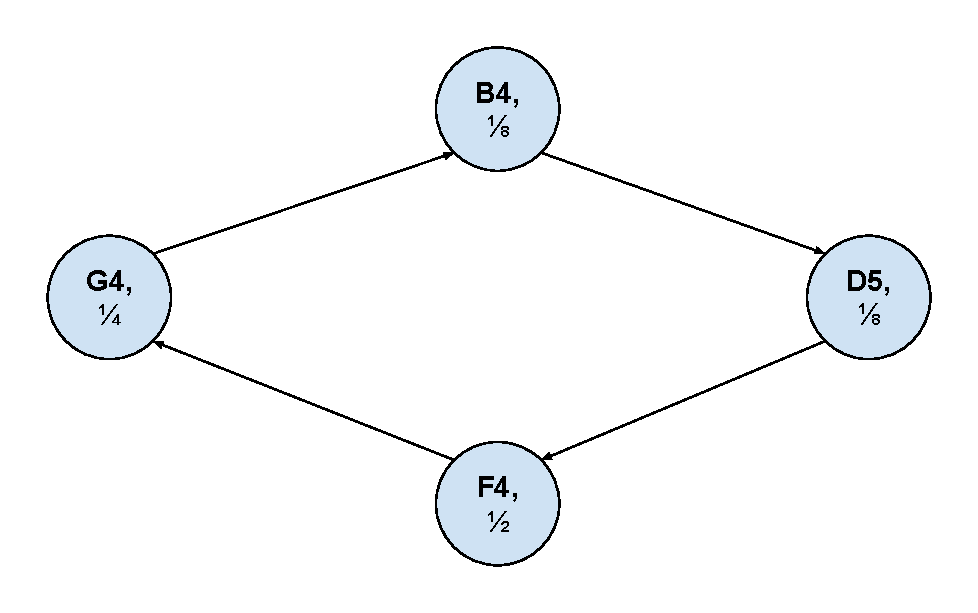
\includegraphics[width=\textwidth]{GraphComposer_4}
%\subcaption*{Second path.}
\end{subfigure}
\end{figure}

En aquest cas, el programa necessita prendre la decisió de quin camí seguir sobre el graf. Aquest mòdul tria de forma aleatoria entre les dues opcions (amb igual probabilitat), i això crea el que s'anomena com a passeigs aleatoris pel graf. Com que la música que produeix cada camí pot resultar en diferents longituds i, per aquest motiu, en una duració diferent de la música. Això pot fer que qui l'escolti la percebi com una mena de ``no-ritme''.

El model utilitzat pel Graph Composer s'utilitza en Musicologia Computacional, un camp d'estudi on les matemàtiques i la informàtica s'apliquen a la música. A la recerca, les composicions musicals es modelen amb grafs per comparar-les i extreure'n diferents propietats matemàtiques. Per exemple, el nombre de vegades que es repeteix la transició d'una nota a una altra, el nombre de vegades que tres o més notes apareixen en el mateix ordre i d'altres.

El Graph Composer passeja pels grafs de forma aleatòria des del vèrtex inicial a través de les arestes dirigides fins que troba un vèrtex amb cap aresta de sortida. Després d'això torna al vèrtex inicial. Quan el programa s'inicia, només pots veure el vèrtex inicial (l'únic que es toca sense cap aresta entrant). Pots arrossegar i afegir més vèrtex, canviar les seves notes, la duració i les decoracions. Tot això es pot fer sense la necessitat de parar la música. La complexitat del graf pot incrementar molt ràpidament a mesura que afegeixes vèrtex. Pots crear patrons al teu graf que creïn motius musicals agradables? Que vagi de gust.


\vfill

Autors del mòdul: Pedro Arthur, Vitor Guerra Rolla, i José Ezequiel Soto Sánchez (Instituto de Matemática Pura y Aplicada, Brazil).
Text: els autors.
